% Reporte con fuente de tamaño 12
\documentclass[12pt]{report}

% Packages
\usepackage[spanish]{babel}
\usepackage{amsmath}
\usepackage{amssymb}
\usepackage{amsthm}
\usepackage{graphicx}
\usepackage{float}
\usepackage{listings}
\usepackage{hyperref}
\usepackage{url}
\usepackage{pgfgantt}
\usepackage[strings]{underscore}
\usepackage{natbib}
\usepackage{fontspec}

\setmainfont{Times New Roman}

\bibliographystyle{plain}

\hypersetup{
    colorlinks=true,
    linkcolor={black},
    filecolor=magenta,      
    urlcolor=cyan,
    pdftitle={Factores que afectan al rendimiento académico},
    pdfpagemode=FullScreen,
}

\setlength{\parindent}{0pt} % Remove paragraph indentation

\begin{document}
\begin{titlepage}
    \begin{center}
        \vspace*{1cm}
 
        \Large\textbf{Factores que afectan al rendimiento académico}
 
        \vspace{0.5cm}
            Trabajo final de inferencia estadística
        \vspace{1.5cm}
 
        \textbf{Antonio Cabrera Landín}
 
        \vfill
             
        Trabajo para el doble grado de\\
        Ingeniería del Software y Matemática Computacional\\
             
        \vspace{0.8cm}
      
        
\includegraphics[width=0.4\textwidth]{figures/logo-u-tad.png}
             
        Inferencia Estadística\\
        U-tad\\
        España\\
        Mayo 2025
             
    \end{center}
 \end{titlepage}

\begin{abstract}
Este estudio analiza el impacto de factores socioacadémicos en el consumo de alcohol y el rendimiento estudiantil, utilizando un dataset de $n=395$ alumnos de educación secundaria. Mediante contrastes paramétricos (\textit{t-tests}, ANOVA) y no paramétricos (Mann-Whitney, Kruskal-Wallis), identificamos que:

\begin{itemize}
    \item Los estudiantes en relaciones románticas presentan mayor consumo los fines de semana (\textit{p} $< 0.05$, test U de Mann-Whitney).
    \item Existe una correlación negativa significativa entre el consumo de alcohol (\texttt{Walc}) y las notas finales (\texttt{G3}) ($\rho = -0.21$, \textit{p} $= 0.002$, Spearman).
    \item No hay diferencias significativas en ausencias (\texttt{absences}) por género (\textit{p} $= 0.18$, t-test para muestras independientes).
\end{itemize}

Los resultados destacan la necesidad de intervenciones educativas diferenciadas según el perfil estudiantil. El análisis incluye visualizaciones (QQ-plots, boxplots) y verificación de supuestos (normalidad, homocedasticidad) para garantizar robustez metodológica.
\end{abstract}


\tableofcontents

\listoffigures

\chapter{Introducción}

El rendimiento académico de los alumnos no se limita solo a lo que ocurre dentro del aula, sino que existen multiples factores externos que impactan en sus resultados escolares: su situación familiar, cuanto tiempo usan redes sociales, cuanto salen con los amigos o incluso si tienen pareja o no.

En este trabajo exploraremos que factores de la vida personal de los alumnos influyen en sus notas. Para ello trabajaremos con el dataset \textit{Student Alcohol Consumption}, el cual está disponible públicamente en \href{https://www.kaggle.com/datasets/uciml/student-alcohol-consumption}{Kaggle}. Los datos provienen de un estudio \cite{Cortez2008} el cual se realizó en dos escuelas secundarias portuguesas. En este, se recopilaron datos sobre las notas académicas de los alumnos en las asignaturas de matemáticas y portugués, además de información sobre la vida personal de cada estudiante. 

En este análisis estadístico, nos centraremos en los datos correspondientes a los alumnos de matemáticas y analizaremos ciertos aspectos de su vida los cuales se asocian de forma significativa con sus niveles de asistencia en clase o sus calificaciones.

\pagebreak

% Primera tabla: Variables demográficas y familiares
\begin{table}[htbp]
\centering
\caption{Descripción de las variables del conjunto de datos (Parte 1: Variables demográficas y familiares)}
\begin{tabular}{lp{8cm}}
\hline
\textbf{Atributo} & \textbf{Descripción (Dominio)} \\
\hline
\textbf{sex} & Sexo del estudiante (binario: femenino o masculino) \\
\textbf{age} & Edad del estudiante (numérico: de 15 a 22 años) \\
\textbf{school} & Escuela del estudiante (binario: Gabriel Pereira o Mousinho da Silveira) \\
\textbf{address} & Tipo de dirección del hogar (binario: urbano o rural) \\
\textbf{Pstatus} & Estado de convivencia de los padres (binario: viven juntos o separados) \\
\textbf{Medu} & Nivel educativo de la madre (numérico: de 0 a 4) \\
\textbf{Mjob} & Trabajo de la madre (nominal: teacher, health, services, at\_home, other) \\
\textbf{Fedu} & Nivel educativo del padre (numérico: de 0 a 4) \\
\textbf{Fjob} & Trabajo del padre (nominal: teacher, health, services, at\_home, other) \\
\textbf{guardian} & Tutor del estudiante (nominal: madre, padre u otro) \\
\textbf{famsize} & Tamaño de la familia (binario: $\leq$ 3 o $>$ 3) \\
\textbf{famrel} & Calidad de las relaciones familiares (numérico: de 1 - muy mala a 5 - excelente) \\
\textbf{reason} & Razón para elegir la escuela (nominal: cercanía al hogar, reputación de la escuela, preferencia por el curso u otro) \\
\textbf{traveltime} & Tiempo de viaje de casa a la escuela (numérico: 1 - $<$15 min, 2 - 15-30 min, 3 - 30 min-1h, 4 - $>$1h) \\
\textbf{internet} & Acceso a Internet en casa (binario: sí o no) \\
\textbf{nursery} & Asistió a educación preescolar (binario: sí o no) \\
\hline
\end{tabular}
\label{tab:variables_parte1}
\end{table}

\pagebreak

% Segunda tabla: Variables académicas y de comportamiento
\begin{table}[htbp]
\centering
\caption{Descripción de las variables del conjunto de datos (Parte 2: Variables académicas y de comportamiento)}
\begin{tabular}{lp{8cm}}
\hline
\textbf{Atributo} & \textbf{Descripción (Dominio)} \\
\hline
\textbf{studytime} & Tiempo de estudio semanal (numérico: 1 - $<$2h, 2 - 2-5h, 3 - 5-10h, 4 - $>$10h) \\
\textbf{failures} & Número de reprobaciones previas (numérico: n si 1$\leq$n$<$3, sino 4) \\
\textbf{schoolsup} & Apoyo educativo adicional de la escuela (binario: sí o no) \\
\textbf{famsup} & Apoyo educativo familiar (binario: sí o no) \\
\textbf{activities} & Actividades extracurriculares (binario: sí o no) \\
\textbf{paidclass} & Clases pagadas adicionales (binario: sí o no) \\
\textbf{higher} & Aspira a educación superior (binario: sí o no) \\
\textbf{romantic} & Tiene una relación romántica (binario: sí o no) \\
\textbf{freetime} & Tiempo libre después de la escuela (numérico: de 1 - muy poco a 5 - mucho) \\
\textbf{goout} & Salidas con amigos (numérico: de 1 - muy pocas a 5 - muy frecuentes) \\
\textbf{Walc} & Consumo de alcohol en fines de semana (numérico: de 1 - muy bajo a 5 - muy alto) \\
\textbf{Dalc} & Consumo de alcohol en días laborales (numérico: de 1 - muy bajo a 5 - muy alto) \\
\textbf{health} & Estado de salud actual (numérico: de 1 - muy malo a 5 - excelente) \\
\textbf{absences} & Número de ausencias escolares (numérico: de 0 a 93) \\
\textbf{G1} & Nota del primer período (numérico: de 0 a 20) \\
\textbf{G2} & Nota del segundo período (numérico: de 0 a 20) \\
\textbf{G3} & Nota final (numérico: de 0 a 20) \\
\hline
\end{tabular}
\label{tab:variables_parte2}
\end{table}


\chapter{Planteamiento del problema}


\chapter{Estado de la cuestión}

El rendimiento escolar ha sido ampliamente estudiado en las últimas décadas, posiblemente por su gran impacto socio-económico en la vida de las personas. Diversos estudios, además de estudiar los factores que pueden controlan los centros educativos, se han centrado en los externos como el entorno familiar, el consumo de sustancias y la relaciones personales de los alumnos.

En este trabajo se seguirá esta línea de investigación, por lo que analizaremos conclusiones previas de otros estudios sobre los factores que recopila nuestro conjunto de datos.

\section{Factores externos que influyen en el rendimiento académico}

Numerosos estudios \cite{mendez2018clima}\cite{sanchez2015entorno} destacan la importancia del entorno familiar para las notas de los estudiantes. En nuestro conjunto de datos contamos con variables como el nivel educativo de los padres (\textit{Medu}, \textit{Fedu}), el estado de convivencia de los padres (\textit{Pstatus}), el apoyo familiar escolar (\textit{famsup}) e incluso la calidad de las relaciones familiares percibida por los alumnos (\textit{famrel}).

Una de las variables que se estudiaran en este trabajo será la de las clases particulares (variable \textit{paid}). En España el refuerzo escolar mediante clases particulares no ha hecho más que aumentar en las últimas décadas \cite{RunteGeidel2013}. Sin embargo, algunos estudios \cite{baker2001worldwide} \cite{wiseman2021does} identificaron una correlación negativa entre las clases particulares 1 a 1 y los logros de los alumnos de matemáticas, sugiriendo que se utiliza más como un remedio que como una solución real.

Uno de los fenómenos más disruptores a nivel social, especialmente en los jóvenes, es el auge de internet. Varios estudios \cite{ramos2017procrastinacion} \cite{vila2018rendimiento} afirman que la adicción y el uso problemático de internet están correlacionados con peor rendimiento académico. Aunque hay que tener en cuenta estudios que sugieren que el acceso a internet puede llegar a favorecer las medias de los alumnos \cite{garcia2022analisis}.

Otros de los factores que analizaremos será el consumo de alcohol de los alumnos. Estudios previos sugieren que el consumo de alcohol a edades tempranas podría afectar al rendimiento escolar así como aumentar el número de faltas en clase \cite{wagner2007alcohol} \cite{kovacs2008relacion}.

En nuestros datos tenemos constancia de si los alumnos son solteros o no. En relación con el consumo de alcohol, un estudio de la universidad de Georgia determinó que los alumnos que tenían más citas reportaban cuatro veces más abandono de los estudios y además se observó en ellos el doble de abuso de sustancias como el alcohol \cite{orpinas2013dating}.

En cuanto a la construcción de modelos para predecir la nota de los alumnos, existen varios estudios que utilizan técnicas de \textit{data mining} y \textit{machine learning} para predecir el rendimiento académico de los alumnos \cite{mengash2020using} \cite{cortez2008using}.

\section{Metodologías utilizadas en estudios previos}

Al ser una materia estudiada desde hace décadas hemos visto una evolución de los métodos empleados. Uno de los mayores motivos es el reconocimiento creciente de la complejidad del problema, en el inicio existía un acuerdo general en como evaluar el rendimiento académico y había mucho mayor consenso en los factores que influenciaban las medias de los alumnos.

En la actualidad, se reconocen factores no cognitivos como la motivación, las aspiraciones académicas o la inteligencia emocional. En general se estudian muchos más factores que podrían influir en el desempeño académico, no solo por una mejora en el análisis del problema sino además por la aparición de nuevos hábitos perjudiciales para el estudiante (redes sociales, videojuegos...).

No solo se ha mejorado en que factores se estudian, sino además en como se estudian. Gracias a los avances en computación a día de hoy se emplean mucho más las técnicas de \textit{data mining} para la construcción de muestras y de \textit{machine learning} para realizar predicciones.

Por último, cabe destacar un aumento en el interés sobre la materia. Gracias a esto, se ha logrado una mayor base geográfica y cultural en la que estudiar el problema, además de tener una mayor cantidad de fuentes y de estudios previos que consultar.


\chapter{Desarrollo, resolución, resultados e interpretación}

\section{¿Aumenta la pareja el número de faltas en clase?}
En nuestro dataset una proporción considerable de alumnos tienen una relación de pareja.

\begin{figure}[H]
    \centering
    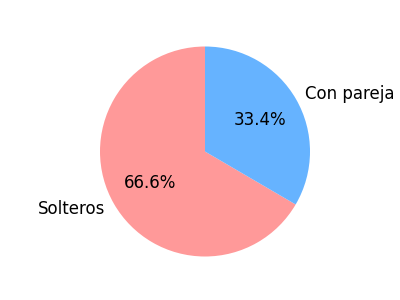
\includegraphics[width=0.6\textwidth]{./figures/proporcion-solteros-pareja.png}
    \caption{Proporción de alumnos solteros vs con pareja}
    \label{fig:prop-solteros}
\end{figure}

\pagebreak

Además, vemos que la edad de los estudiantes está comprendida entre los 15 y 22 años. Podemos suponer que en estas edades las relaciones románticas tienen mucho impacto en la vida escolar, en concreto en la asistencia en clase.
\begin{figure}[H]
    \centering
    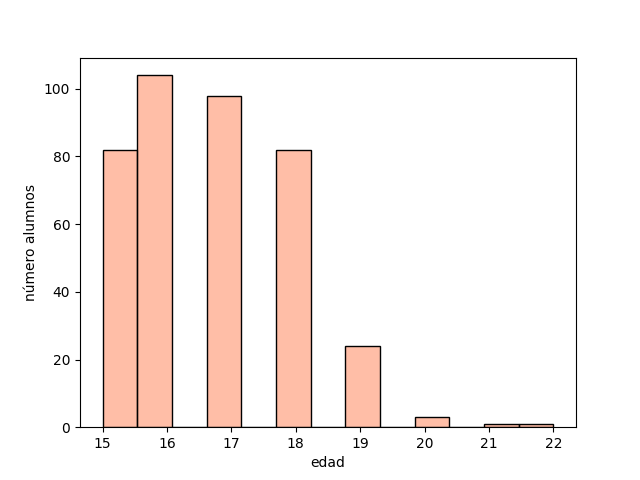
\includegraphics[width=0.8\textwidth]{./figures/edad-alumnos.png}
    \caption{Histograma de las edades de los alumnos}
    \label{fig:hist-edad}
\end{figure}

Por lo tanto, con el objetivo de estudiar que factores de la vida personal de los alumnos influyen en sus notas escolares, vamos a comenzar contrastando si tener pareja aumenta el número de faltas en clase.
\begin{equation*}
    \begin{split}
        & X \equiv \text{Número de faltas en clase de los alumnos con pareja}\\
        & Y \equiv \text{Número de faltas en clase de los alumnos solteros}
    \end{split} 
\end{equation*}

\pagebreak

Para poder elegir un contraste de hipótesis, primero debemos estudiar la distribución de los datos.

Viendo los gráficos de distribución de el número de faltas en clase de los alumnos con pareja y solteros podemos asumir que los datos no provienen de una población normal, ya que en ambos casos son datos muy asimétricos.

\begin{figure}[H]
    \centering
    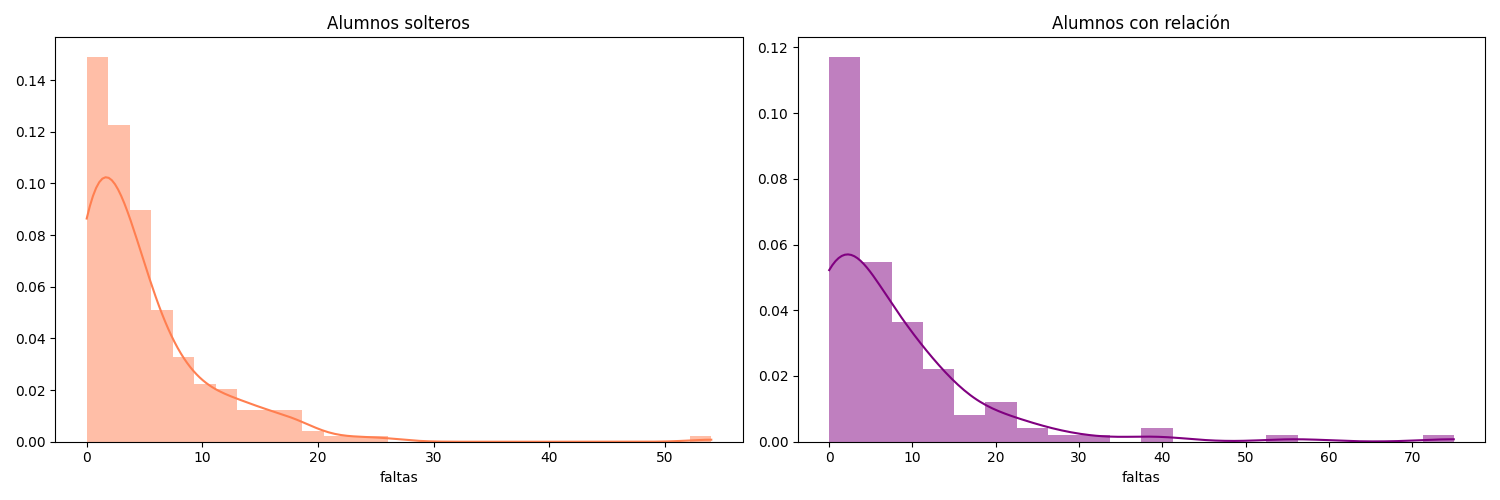
\includegraphics[width=1\textwidth]{./figures/distribucion-numero-faltas.png}
    \caption{Gráficos de distribución del número de faltas de los alumnos}
    \label{fig:dist-num-faltas}
\end{figure}

Para asegurarnos de que estamos en lo correcto realizaremos un contraste de normalidad. En nuestro caso utilizaremos el test Ómnibus d´Agostino, ya que nuestros datos cumplen con el requisito de tener más de 20 entradas ($n>20$).

Realizaremos el test tanto para alumnos solteros como para alumnos con pareja. Las hipótesis para los alumnos solteros serían las siguientes:

\begin{itemize}
    \item \textbf{Hipótesis nula ($H_0$)}: $X \sim N(\mu, \sigma)$ (Los datos del número de faltas en alumnos con pareja siguen una distribución normal)
    \item \textbf{Hipótesis alternativa ($H_a$)}: $X \not \sim N(\mu, \sigma)$ (Los datos del número faltas en alumnos con pareja no sigue una distribución normal)
\end{itemize}

\pagebreak

En el caso de los alumnos con pareja al calcular el estadístico de contraste observado obtenemos $K^2_x = 116.45$ y al calcular el p-valor obtenemos un valor muy cercano al cero.

\begin{equation*}
    \text{p-valor} = P(K^2_x > 116.45) \approx 0
\end{equation*}

Por lo tanto, en el caso de los alumnos solteros, los datos muestran evidencias suficientes para rechazar la hipótesis nula de que el número de faltas en la muestra sigue una distribución normal.

En el caso de los alumnos con pareja obtendremos las mismas conclusiones, por lo que aceptaremos la no-normalidad de los datos en ambos casos.
\pagebreak

Como asumimos que los datos no provienen de una distribución normal utilizaremos un contraste no paramétrico. Como estamos trabajando con muestras independientes, elegiremos el contraste U de Mann-Whitney.

Para ello plantearemos las siguientes hipótesis:

\begin{itemize}
    \item \textbf{Hipótesis nula ($H_0$)}: $\mu_x = \mu_y$ (No existe una diferencia significativa entre el número de faltas medio entre los alumnos con pareja y solteros)
    \item \textbf{Hipótesis alternativa ($H_a$)}: $\mu_x > \mu_y$ (El número de faltas medio en los alumnos con pareja es mayor que el de los alumnos solteros)
\end{itemize}

Al calcular es estadístico de contraste $U$ obtenemos un valor observado de 18787.5, el cual sugiere diferencias pequeñas entre ambas poblaciones.
\begin{equation*}
    \text{p-valor} = P(U > 18787.5) = 0.0874 > \alpha 
\end{equation*}

Viendo que el p-valor supera nuestro nivel de significación $\alpha$ de 0.05, podemos afirmar que al $5\%$ los datos no muestran evidencias suficientes como para rechazar la hipótesis de que no exista una diferencia significativa entre el número de faltas medios de los alumnos solteros y con pareja.

Este resultado es sorprendente ya que la media faltas en solteros es de $4.84$ faltas y en alumnos con pareja es de $7.44$ faltas. 
\begin{equation*}
    \begin{split}
        & \bar{x} = 7.44\\
        & \bar{y} = 4.84
    \end{split}
\end{equation*}

Pero en definitiva, aceptamos que el hecho de tener pareja no afecta significativamente al número de faltas medio a lo largo del curso.

\pagebreak
\section{¿Mejoran las notas a lo largo del curso?}

Un indicio de un buen sistema educativo es el de que los alumnos mejoran sus notas a lo largo del curso. En nuestros datos tenemos registros de las notas de los estudiantes a lo largo del curso, por lo tanto podemos contrastar si existe un progreso. Para ello contrastaremos si la nota media del primer periodo $G_{1}$ y la nota media final $G_{3}$ difieren significativamente.
\begin{equation*}
    \begin{split}
        & X \equiv \text{Nota de los alumnos en el primer periodo}\\
        & Y \equiv \text{Nota final de los alumnos}
    \end{split} 
\end{equation*}

Esta vez vemos que los gráficos de distribución de las notas del primer periodo y del final se asemejan más al de la distribución normal.

\begin{figure}[H]
    \centering
    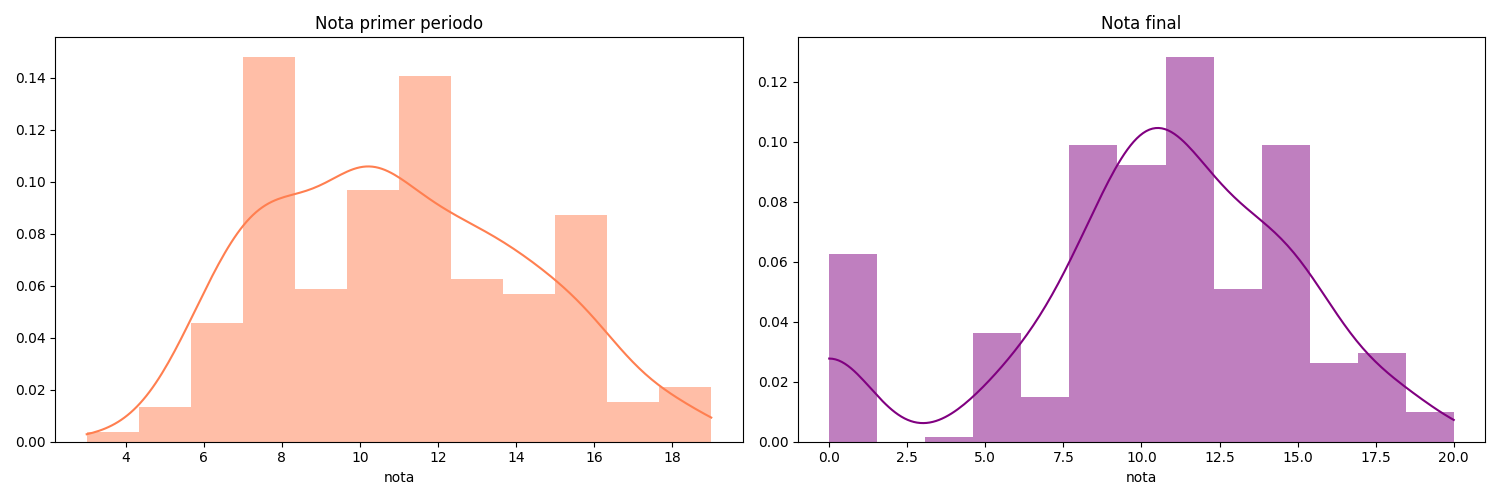
\includegraphics[width=1\textwidth]{./figures/dist-notas-alumnos.png}
    \caption{Gráficos de distribución de las notas de los alumnos}
    \label{fig:dist-notas}
\end{figure}

Si volvemos a realizar el test de Ómnibus d´Agostino obtenemos los siguientes resultados:
\begin{equation*}
    \begin{split}
        & K^2_{x} = 22.61 \Rightarrow \text{p-valor} = P(K^2 > 22.61) \approx 0\\ 
        & K^2_{y} = 32.05 \Rightarrow \text{p-valor} = P(K^2 > 32.05) \approx 0
    \end{split}
\end{equation*}

Aunque los estadísticos observados son más pequeños (denotando que las muestras son más anteriores que cuando veíamos las faltas en clase), los p-valores siguen siendo muy cercanos al cero.

\pagebreak

Sin embargo, como los datos son medianamente simétricos y además disponemos de una muestra suficientemente grande, utilizaremos un contraste paramétrico de diferencia de medias.
\begin{equation*}
    \begin{split}
        & \gamma_{1}(x) = \frac{\sum_{i=1}^{n}(x_i - \bar{x})^3}{n \cdot s^3} = 0.24\\
        & \gamma_{1}(y) = \frac{\sum_{i=1}^{n}(y_i - \bar{y})^3}{n \cdot s^3} = -0.73
    \end{split} 
\end{equation*}

Como estamos trabajando con muestras dependientes (medimos la nota del alumno en distintos momentos y además la nota final depende de la nota del primer y segundo periodo), utilizaremos un t-test de muestras pareadas.
\begin{itemize}
    \item \textbf{Hipótesis nula ($H_0$)}: $\mu_x - \mu_y = \mu_D = 0$ (no existe diferencias significativas entre la nota media del primer periodo y la nota media final)
    \item \textbf{Hipótesis alternativa ($H_a$)}: $\mu_x - \mu_y = \mu_D > 0$ (la nota media final mejora significativamente respecto a la nota media del primer periodo)
\end{itemize}

Al realizar el test obtenemos los siguientes resultados:
\begin{equation*}
    t_{obs} = 3.55 \Rightarrow \text{p-valor} = P(t_{394} > 3.55) = 0.0002
\end{equation*}

Por lo tanto, viendo que el p-valor es pequeño, concluimos que los datos muestran evidencias suficientes como para rechazar que la diferencia entre la media del primer periodo y la media final no es significativa. Aceptaremos la hipótesis alternativa de que la media final aumenta respecto a la del primer periodo.

\pagebreak
\section{¿Ayudan las clases particulares a aprobar?}

Muchas familias recurren a las clases particulares cuando sus hijos no consiguen aprobar los exámenes. Estudiaremos si realmente son efectivas.
\begin{equation*}
    \begin{split}
        & X \equiv \text{Nota final de los alumnos que asisten a clases particulares}\\
        & Y \equiv \text{Nota final de los alumnos no que asisten a clases particulares}
    \end{split}
\end{equation*}

En nuestros datos, un $71.82\%$ de los alumnos que tomaron clases particulares aprobaron. En comparación, un $63.08\%$ de los alumnos que no fueron a clases particulares aprobaron.
\begin{equation*}
    \begin{split}
        & p_{x} = 0.7182\\
        & p_{y} = 0.6308
    \end{split}
\end{equation*}

Como en los contrastes anteriores, primero tenemos que estudiar la normalidad de la población.

\begin{figure}[H]
    \begin{center}
        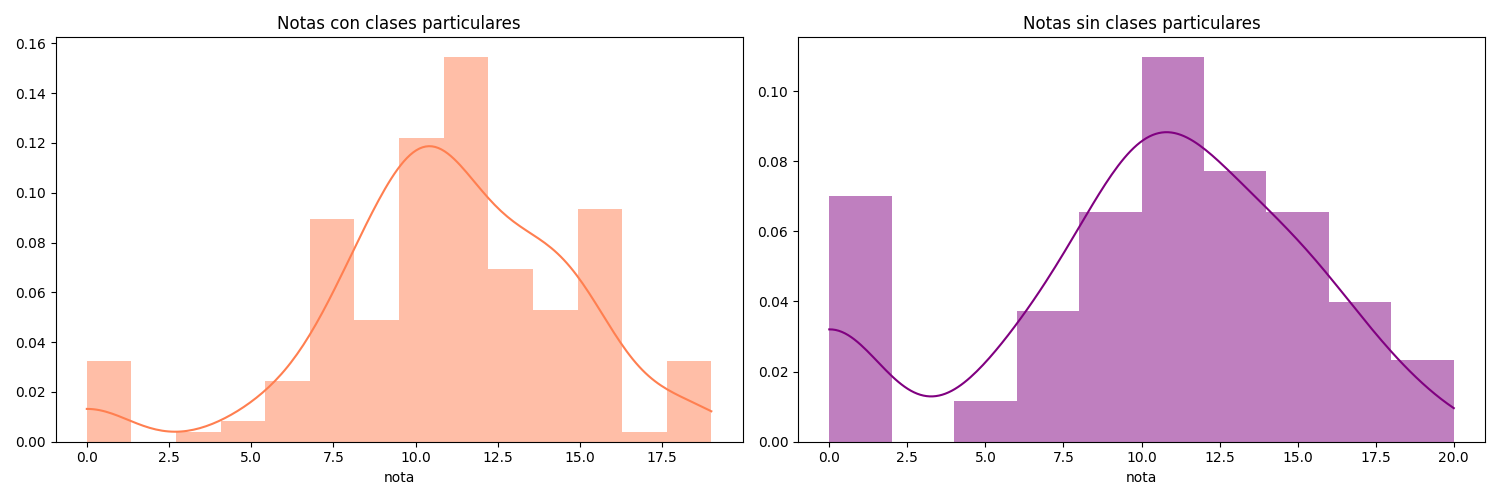
\includegraphics[width=1\textwidth]{figures/dist-notas-clases-particulares.png}
    \end{center}
    \caption{Gráficos de distribución de las notas finales de los alumnos que toman clases particulares y de los que no}
    \label{fig:dist-notas-clases-particulares}
\end{figure}

Esta vez, nos ayudaremos del QQ-plot, el cual compara los cuantiles observados con los cuantiles teóricos de la distribución normal.

\begin{figure}[H]
    \begin{center}
        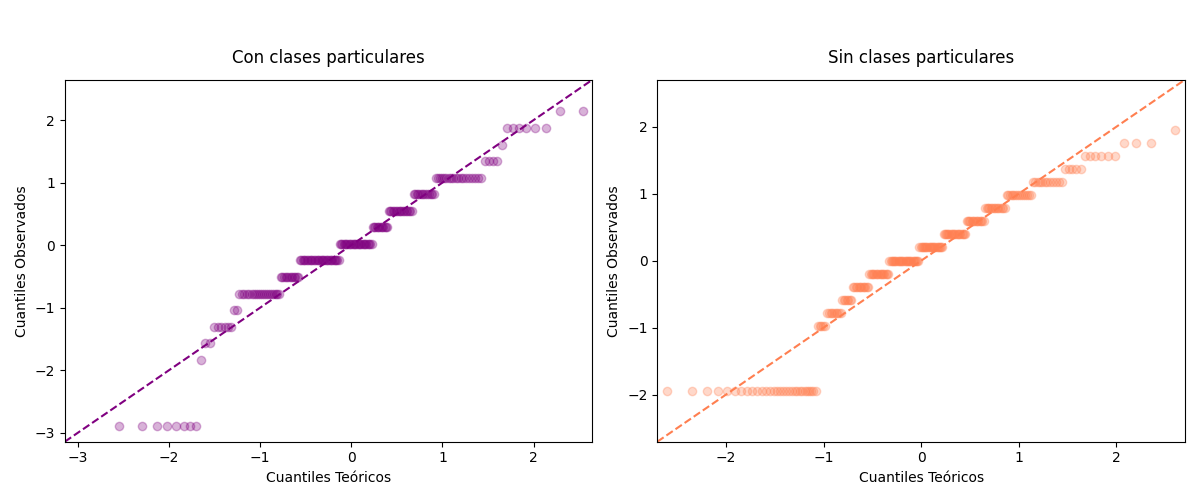
\includegraphics[width=1\textwidth]{figures/qq-plot-notas-particulares.png}
    \end{center}
    \caption{QQ-plot de las notas finales de alumnos que toman clases particulares y de los que no}\label{fig:qq-plot}
\end{figure}

Vemos que en ambos gráficos, los cuantiles se ajustan bien excepto al comienzo. Esto se debe a que hay muchos alumnos con ceros en la nota ya que no se presentaron a clase. 

Como estamos trabajando con muestras grandes y los datos presentan una asimetría moderada, utilizaremos un contraste paramétrico para la diferencia de proporciones.

\begin{equation*}
    \begin{split}
        & \gamma_{1}(x) = \frac{\sum_{i=1}^{n}(x_i - \bar{x})^3}{n \cdot s^3} = -0.70\\
        & \gamma_{1}(y) = \frac{\sum_{i=1}^{n}(y_i - \bar{y})^3}{n \cdot s^3} = -0.61
    \end{split} 
\end{equation*}

Nuestras hipótesis serán las siguientes:

\begin{itemize}
    \item \textbf{Hipótesis nula ($H_0$)}: $\pi_{x} - \pi_{y} = 0$ (no existe diferencias significativas entre las proporciones de aprobados entre los alumnos que asisten a clases particulares y de los que no)
    \item \textbf{Hipótesis alternativa ($H_a$)}: $\pi_{x} - \pi_{y} > 0$ (la proporción de aprobados de los alumnos que toman clases particulares es mayor respecto a la de los alumnos que no)
\end{itemize}

Al realizar el test obtenemos los siguientes resultados:
\begin{equation*}
    Z_{\text{obs}} = 1.8417 \Rightarrow \text{p-valor} = P(Z > 1.8417) = 0.0328
\end{equation*}

Con un $5\%$ de significación, diremos que los datos muestran evidencias suficientes como para rechazar que las proporciones de aprobados en los alumnos que toman clases particulares y de los que no no difieren significativamente. Por lo tanto, al $5\%$, aceptaremos la hipótesis alternativa de que la proporción de aprobados es mayor en los alumnos que asisten a clases particulares.

\pagebreak
\section{¿Aumenta el acceso a internet la variabilidad de la nota?}

Internet puede ser una poderosa herramienta para el aprendizaje de los alumnos, aportando una cantidad inmensurable de materiales didácticos de forma gratuita. Sin embargo, también trae consigo las redes sociales, a las cuales se les atribuye varios efectos adversos como la perdida la de atención.

\begin{equation*}
    \begin{split}
        & X \equiv \text{Nota final de los alumnos con acceso a internet}\\
        & Y \equiv \text{Nota final de los alumnos sin acceso a internet}
    \end{split}
\end{equation*}
    
En nuestros datos vemos que las varianzas muestrales varían en una unidad. Veremos si estas observaciones son atribuibles al azar.
\begin{equation*}
    \begin{split}
        & S_x^2 = 20.92\\
        & S_{y}^2 = 19.82
    \end{split}
\end{equation*}

Antes de elegir el test, debemos comprobar la normalidad de los datos para ver si elegimos un contraste paramétrico o no paramétrico.

\begin{figure}[H]
    \begin{center}
        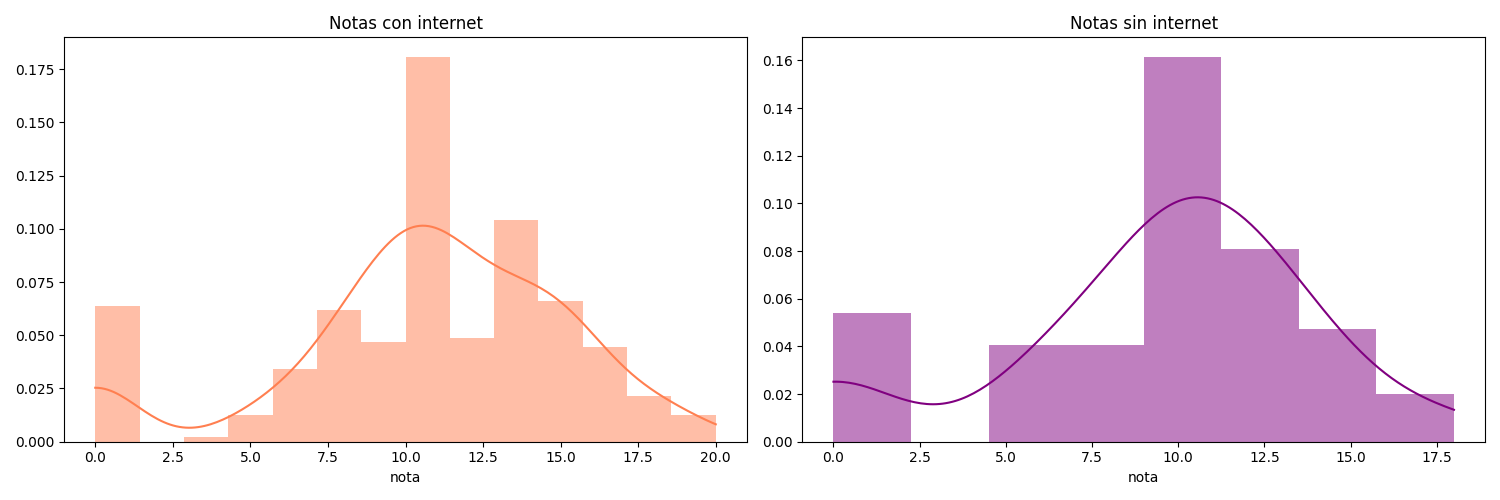
\includegraphics[width=1\textwidth]{figures/dist-notas-internet.png}
    \end{center}
    \caption{Distribución de las notas finales con y sin internet}\label{fig:dist-notas-internet}
\end{figure}

Como en casos anteriores, utilizaremos el test de Ómnibus d´Agostino.
\begin{equation*}
    \begin{split}
        & K_{x}^2 = 28.77 \Rightarrow \text{p-valor} = P(K^2 > 28.77) \approx 0\\
        & K_{y}^2 = 6.15 \Rightarrow \text{p-valor} = P(K^2 > 6.15) = 0.046
    \end{split}
\end{equation*}

En ambos casos, al $5 \%$, rechazaríamos la hipótesis nula de normalidad.

Aunque nuestros datos tienen asimetría negativa moderada y son muestras grandes, el contraste $F$ de diferencia de varianzas es muy sensible a la no-normalidad de los datos. Por lo tanto, viendo que los datos muestran evidencias suficientes como para rechazar la normalidad, nos decantaremos por un test no-paramétrico.
\begin{equation*}
    \begin{split}
        & n_{1} = 329\\
        & n_{2} = 66
    \end{split}
\end{equation*}
\begin{equation*}
    \begin{split}
        & \gamma_{1}(x) = \frac{\sum_{i=1}^{n}(x_i - \bar{x})^3}{n \cdot s^3} = -0.75\\
        & \gamma_{1}(y) = \frac{\sum_{i=1}^{n}(y_i - \bar{y})^3}{n \cdot s^3} = -0.71
    \end{split} 
\end{equation*}

Aplicaremos un contraste de Levene de igualdad de varianzas.

\begin{itemize}
    \item \textbf{Hipótesis nula ($H_0$)}: $\sigma_{x}^2 = \sigma_{y}^2$ (no existen diferencias significativas entre la varianza de las notas de los alumnos con internet y los alumnos sin internet)
    \item \textbf{Hipótesis alternativa ($H_a$)}: $\sigma_{x}^2 \neq \sigma_{y}^2$ (existen diferencias significativas entre la varianza de las notas de los alumnos con internet y los alumnos sin internet)
\end{itemize}

Al calcular el estadístico de contraste $W$ obtenemos los siguientes resultados:
\begin{equation*}
    W = 0.17 \Rightarrow P(F_{k-1,N-k} > W) = P(F_{1, 393} > 0.17) = 0.68
\end{equation*}

Entonces, como hemos obtenido un p-valor alto, los datos son compatibles con la hipótesis nula de igualdad de varianzas. Los datos no muestran evidencias suficientes como para rechazar que las varianzas en las notas de los alumnos con y sin internet sean iguales. Por lo tanto, aceptaremos que el hecho de tener internet no influye en la variabilidad de la nota.

\pagebreak
\section{¿Afecta en la nota el consumo de alcohol?}

En nuestra muestra hay 244 alumnos que consumen alcohol los fines de semana (un 62\%), de los cuales la media de edad es de $16.8$ años (es decir, la mayoría son menores). Es probable que en estas edades los alumnos aun no gestionen bien el consumo de alcohol y es posible que esto repercuta en sus notas finales.
\begin{equation*}
    \begin{split}
        & X \equiv \text{Nota final de los alumnos que consumen alcohol los fines de semana}\\
        & Y \equiv \text{Nota final de los alumnos que no consumen alcohol los fines de semana}
    \end{split}
\end{equation*}

En nuestros datos si que observamos un descenso en la nota media de los alumnos que consumen alcohol.
\begin{equation*}
    \begin{split}
        & \bar{x} = 10.22\\
        & \bar{y} = 10.74
    \end{split}
\end{equation*}

\begin{figure}[H]
    \begin{center}
        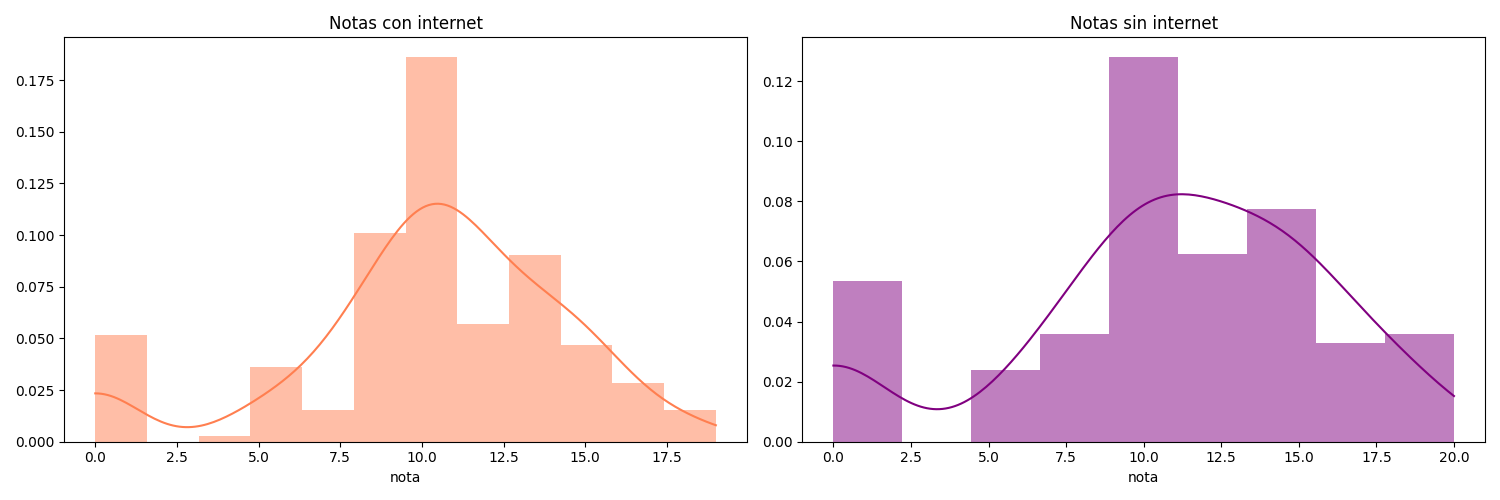
\includegraphics[width=1\textwidth]{figures/dist-notas-walc.png}
    \end{center}
    \caption{Gráficos de distribución de la nota final de los alumnos que consumen alcohol los fines de semana y de los que no}\label{fig:dist-notas-walc}
\end{figure}

Si estudiamos el QQ-plot de las notas finales de ambos grupos, obtendremos resultados similares al anterior: existen muchos \textit{outliers} de los alumnos que no se presentaron al examen final.
\begin{figure}[H]
    \begin{center}
        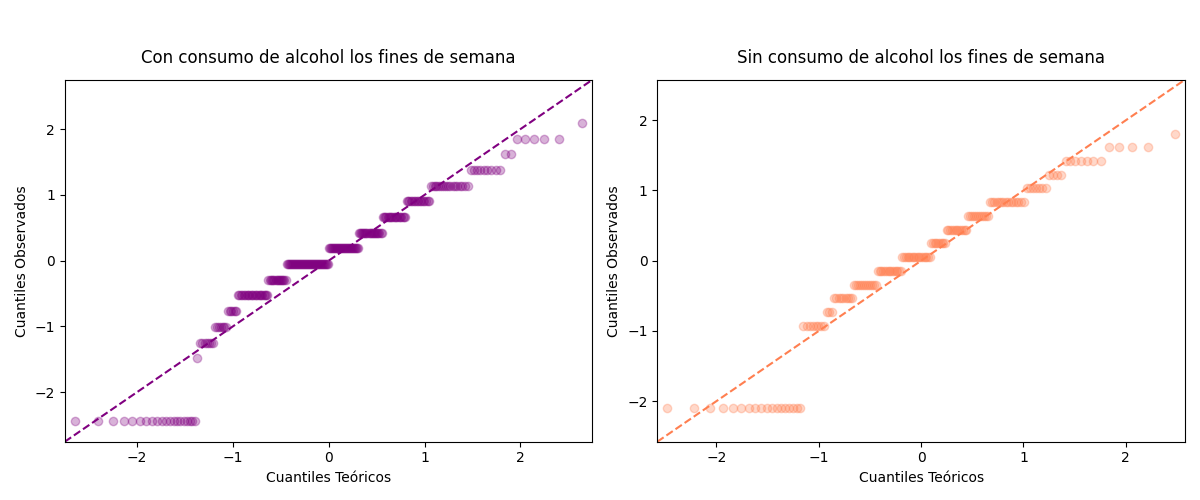
\includegraphics[width=1\textwidth]{figures/qq-plot-walc.png}
    \end{center}
    \caption{QQ-plot de la nota final de los alumnos que consumen alcohol los fines de semana y de los que no}\label{fig:qq-plot-walc}
\end{figure}

Si comprobamos la asimetría de la muestras veremos que es moderada en ambos casos.
\begin{equation*}
    \begin{split}
        & \gamma_{1}(x) = \frac{\sum_{i=1}^{n}(x_i - \bar{x})^3}{n \cdot s^3} = -0.82\\
        & \gamma_{1}(y) = \frac{\sum_{i=1}^{n}(y_i - \bar{y})^3}{n \cdot s^3} = -0.70
    \end{split} 
\end{equation*}

Por lo tanto, como además estamos trabajando con muestras grandes e independientes, utilizaremos un contraste paramétrico de diferencia de medias para muestras grandes independientes con varianzas poblacionales desconocidas (Z test).
\begin{itemize}
    \item \textbf{Hipótesis nula ($H_0$)}: $\mu_x - \mu_y = 0$ (no existen diferencias significativas entre la media de las notas finales de los alumnos que consumen alcohol los fines de semana y de los que no)
    \item \textbf{Hipótesis alternativa ($H_a$)}: $\mu_x - \mu_y < 0$ (la nota media de los alumnos que consumen alcohol los fines de semana es significativamente menor que la de los alumnos que no consumen)
\end{itemize}

Al calcular el estadístico de contraste $Z_{\text{obs}}$, obtenemos el siguiente p-valor.
\begin{equation}
    Z_{\text{obs}} = -1.09 \Rightarrow \text{p-valor} = P(Z < -1.09) = 0.14
\end{equation}

Si fijamos un nivel de significación $\alpha = 0.05$ (el error de tipo 1 máximo que permitimos en nuestro contraste), entonces $\text{p-valor} > \alpha$ lo que significa que al 5\% los datos no dan evidencias suficientes como para rechazar que las medias de las notas finales de los alumnos que consumen y no consumen alcohol los fines de semana sean iguales. Por lo tanto, al 5\% aceptaremos que las notas medias de los alumnos que toman y no toman alcohol no difieren significativamente.



\chapter{Conclusiones}

Este estudio ha explorado diversos factores externos que influyen en el rendimiento académico de estudiantes de secundaria, utilizando técnicas estadísticas para contrastar hipótesis y un modelo predictivo para evaluar su impacto conjunto.

\section{Resultados del trabajo}

A continuación, se resumen las principales conclusiones derivadas de los análisis realizados:  

\begin{enumerate}
    \item \textbf{Relaciones románticas y asistencia a clase}

    Aunque los alumnos con pareja presentaron un mayor número medio de faltas (7,44 frente a 4,84 en solteros), el contraste de Mann-Whitney no mostró diferencias significativas al 5\% de significación. Esto sugiere que, a pesar de la percepción generalizada, tener pareja no afecta significativamente a la asistencia escolar. 
    \item \textbf{Evolución de las notas a lo largo del curso}

    El análisis confirmó que las notas mejoran significativamente del primer período (G1) al final (G3), respaldando la efectividad del sistema educativo evaluado.

    \item \textbf{Clases particulares y probabilidad de aprobar}

    Los alumnos que recibieron clases particulares tuvieron una tasa de aprobados mayor (71,82\%) frente a quienes no las tomaron (63,08\%). El contraste de proporciones mostró que esta diferencia es estadísticamente significativa al 5\%, lo que respalda la utilidad de las clases de refuerzo. Sin embargo, como ya hemos visto, estudios previos \cite{baker2001worldwide} \cite{wiseman2021does} dudan de la efectividad real de las clases particulares tradicionales.

    \item \textbf{Acceso a internet y variabilidad en las notas}

    El acceso a internet no mostró un impacto significativo en la dispersión de las calificaciones, según el contraste de Levene. Una hipótesis puede ser que en la escuela del conjunto de datos no está extendida la adicción a internet, ya que como hemos visto en otros estudios \cite{vila2018rendimiento}, el uso problemático de internet puede conllevar un impacto significativo en las notas de los alumnos.

    \item \textbf{Consumo de alcohol y rendimiento académico}

    A pesar de que el 62\% de los alumnos consumía alcohol los fines de semana, no se encontró una diferencia significativa en las notas medias respecto a los no consumidores. Este resultado contrasta con investigaciones previas que vinculan el consumo temprano de alcohol con bajo rendimiento \cite{wagner2007alcohol}.
\end{enumerate}

    Respecto al modelo LOGIT desarrollado existe mucho margen de mejora. Al realizar el contraste de significancia de sus parámetros, vimos que no elegimos las mejores variables para predecir si los alumnos aprueban o suspenden. Además, solo tuvimos en cuenta 4 de las 30 variables de las que disponemos en el dataset.   

\section{Reflexiones finales}

Los resultados subrayan que el rendimiento académico es multifactorial y no puede atribuirse únicamente a variables aisladas. Factores como las clases particulares y la asistencia a clase demostraron tener un impacto tangible, mientras que otros (relaciones románticas, internet o alcohol) no fueron concluyentes en este contexto. Esto nos alerta de no solo fijarnos en los factores internos de los centros educativos, sino además tener más en cuenta los externos para poder desarrollar soluciones académicas más efectivas

\section{Limitaciones y futuras líneas de investigación}

\begin{itemize}
    \item La muestra proviene de un contexto geográfico y cultural específico (Portugal), lo que limita la generalización.  
    \item Algunas de las variables cualitativas pueden estar sesgadas (por ejemplo cuando se les pregunta a los alumnos por sus relaciones familiares).
    \item Se podrían utilizar técnicas de \textit{machine learning} para predecir las notas de los alumnos.
\end{itemize}

La mayor limitación de este trabajo quizá sea la falta de extensión y de estudio de los datos. Solo hemos conseguido abarcar 5 de las 30 variables del conjunto de datos, además se podría indagar mucho más en análisis de cada una de ellas.

\section{Reflexión personal}

En lo personal, este trabajo ha sido un valioso acercamiento al mundo académico de la estadística y me ha servido para ver las aplicaciones reales de la inferencia estadística para acercarnos a las verdades de los problemas que afectan a nuestra era.


\bibliography{bibliografia}

\end{document}
